\mychapter{Resultados} 
\label{Cap:Resultados}

Neste capítulo, são apresentados os resultados da implementação e testes do \textit{software} RADARE, com foco na precisão dos dados reconciliados, no desempenho computacional em diferentes cenários de carga e na usabilidade da ferramenta, tanto no \textit{front-end} (menu e \textit{canvas}) quanto no \textit{back-end} (rotas, serviços e banco de dados). Além disso, foram desenvolvidos dois manuais: um para a manutenção técnica do sistema e outro para orientar o uso pelos usuários finais.

Para facilitar a leitura e não quebrar a dinâmica do texto principal, todos os códigos desenvolvidos para o RADARE foram incluídos nos Apêndices. Devido à sua extensão, a decisão de alocar os trechos de código nos Apêndices permite uma melhor fluidez no corpo do trabalho. Sempre que um código for citado ao longo do texto, será indicada a referência ao apêndice correspondente para consulta detalhada.

% -------------------------
\section{Resultados do desenvolvimento do \textit{front-end}} 

O \textit{front-end} do projeto  foi desenvolvido com foco em oferecer uma interface intuitiva, visando otimizar a interação dos usuários com a ferramenta de modelagem. A interface facilita a visualização dos fluxos de dados e dos modelos, além de permitir a execução da reconciliação. O  \textit{front-end} do sistema é estruturado em duas áreas principais: o menu, responsável pelo gerenciamento das ações e funcionalidades, e o \textit{canvas}, onde os nódulos conectados podem ser visualizados e manipulados diretamente pelos usuários.

% -------------------------
\subsection{Menu de controle da interface gráfica} 

A sessão de menu do RADARE apresenta ao usuário uma interface de fácil interação, permitindo a adição de componentes, o controle do fluxo de dados e o gerenciamento da visualização geral do sistema. Cada funcionalidade disponível no menu é descrita de maneira detalhada nas subseções a seguir, acompanhada por exemplos de código e imagens que ilustram sua implementação no contexto da ferramenta.

A biblioteca \textit{ReactFlow} \cite{reactflow} é fundamental para a manipulação dos nódulos no \textit{canvas} e foi significativamente adaptada para atender às necessidades específicas do projeto. As modificações realizadas garantem uma usabilidade eficiente, permitindo que os usuários adicionem e conectem os nódulos de forma dinâmica, com fluidez e precisão.

Cada nódulo inserido no \textit{canvas} possui uma estrutura personalizada, onde as conexões, denominadas \textit{handles}, são configuradas com características específicas, como estilo visual e lógica de interação. Essa personalização assegura que a visualização dos fluxos de dados seja clara e que sua manipulação seja intuitiva, facilitando o gerenciamento das operações dentro do sistema.

A Figura \ref{Fig:MenuImage} apresenta o menu principal do sistema, destacando as opções para adição de nódulos ao \textit{canvas}. Através desse menu, o usuário pode inserir diferentes tipos de nódulos, como entradas, saídas e pontos de processamento de dados, além de opções como reconciliação de dados e ajustes de visualização. Cada funcionalidade foi projetada para que o usuário possa construir fluxos de dados industriais de maneira modular e interativa, proporcionando maior flexibilidade no gerenciamento e análise de grandes volumes de dados.

\begin{figure}[htbp]
    \centering
    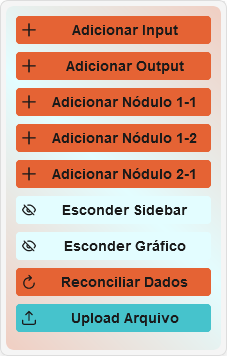
\includegraphics[width=0.4\textwidth]{figuras/menu-image.png}
    \caption{Menu principal do sistema RADARE.}
    \label{Fig:MenuImage}
\end{figure}

\subsubsection{Adicionar Input}

O botão \textbf{"Adicionar Input"} permite ao usuário inserir um novo nódulo de entrada no \textit{canvas}, representando um sensor ou uma fonte de dados no sistema industrial. Ao acionar esse botão, um nó de \textit{input} é adicionado ao \textit{canvas}, possibilitando a conexão desse ponto com outros nódulos do fluxo de dados. A implementação dessa funcionalidade utiliza a biblioteca ReactFlow \cite{reactflow}, o que elimina a necessidade de configurações customizadas iniciais e facilita a criação e manipulação dos nódulos no ambiente visual.

A Figura \ref{Fig:AddInputButton} ilustra o botão "Adicionar Input" na interface gráfica do sistema.

\begin{figure}[htbp]
    \centering
    
\includegraphics[width=0.4\textwidth]{figuras/add-input-button.png}
    \caption{Botão de adicionar input no menu (Fonte: próprio autor, 2024).}
    \label{Fig:AddInputButton}
\end{figure}


\subsubsection{Adicionar output}

O botão \textbf{"Adicionar Output"} permite ao usuário inserir um novo nódulo de saída no \textit{canvas}. Esse \textit{output} representa um destino ou ponto final para os dados no sistema industrial, como a exportação de resultados processados ou a visualização de dados reconciliados. Ao acionar o botão, um novo nó de \textit{output} é adicionado ao \textit{canvas}, possibilitando sua conexão com outros nódulos de processamento ou entrada no fluxo de dados. Assim como ocorre com o \textit{input}, a implementação dessa funcionalidade também utiliza a biblioteca ReactFlow \cite{reactflow}, eliminando a necessidade de customização de comportamentos iniciais.

A Figura \ref{Fig:AddOutputButton} mostra o botão "Adicionar Output" na interface, permitindo ao usuário inserir nódulos de saída no fluxo de dados.

\begin{figure}[htbp]
    \centering
    
\includegraphics[width=0.4\textwidth]{figuras/add-output-button.png}
    \caption{Botão de adicionar output no menu (Fonte: próprio autor, 2024).}
    \label{Fig:AddOutputButton}
\end{figure}

\subsubsection{Adicionar nódulo 1-1}

O botão \textbf{"Adicionar Nódulo 1-1"} permite ao usuário inserir um novo nódulo de transição no \textit{canvas}. Esse nódulo atua como um ponto intermediário no fluxo de dados, podendo representar sensores, transformações ou outros elementos de processo. Ao clicar no botão, o nódulo é adicionado ao \textit{canvas}, permitindo ao usuário conectá-lo com outros nódulos de forma eficiente.

A lógica para adicionar este nódulo foi desenvolvida de forma personalizada, especificando o tipo de conexão, a quantidade de pontos de conexão (\textit{handles}), além do estilo visual e da posição no \textit{canvas}, garantindo que o comportamento do nódulo se ajuste adequadamente ao fluxo de dados esperado.

O trecho principal do código responsável pela criação desse nódulo, que pode ser encontrado em sua totalidade no \textbf{Apêndice \ref{Cap:frontCodeNodeOneOne}}.

A Figura \ref{Fig:AddNodeOneOneButton} ilustra o botão "Adicionar Nódulo 1-1" disponível no menu do sistema.

\begin{figure}[htbp]
    \centering
    
\includegraphics[width=0.4\textwidth]{figuras/add-node11-button.png}
    \caption{Botão de adicionar Nódulo 1-1 no menu (Fonte: próprio autor, 2024).}
    \label{Fig:AddNodeOneOneButton}
\end{figure}


\subsubsection{Adicionar nódulo 1-2}

O botão \textbf{"Adicionar Nódulo 1-2"} permite ao usuário inserir um nódulo de transição que recebe uma única entrada e gera duas saídas no \textit{canvas}. Este tipo de nódulo é particularmente útil em cenários onde um único ponto de dados precisa ser bifurcado para diferentes processos ou análises. Ao ser adicionado, o nódulo facilita o roteamento de dados para dois fluxos distintos, mantendo a integridade e a flexibilidade do processo.

A lógica para este nódulo foi customizada para suportar uma conexão de entrada e duas saídas, com o código responsável definindo os \textit{handles} (pontos de conexão), a posição e o estilo visual no \textit{canvas}. Assim como no caso do nódulo 1-1, o comportamento é ajustado para garantir uma integração fluida no fluxo de dados.

O trecho principal do código responsável pela criação desse nódulo pode ser encontrado em sua totalidade no \textbf{Apêndice \ref{Cap:frontCodeNodeOneTwo}}.

A Figura \ref{Fig:AddNodeOneTwoButton} ilustra o botão "Adicionar Nódulo 1-2" disponível no menu do sistema.

\begin{figure}[htbp]
    \centering
    
\includegraphics[width=0.4\textwidth]{figuras/add-node12-button.png}
    \caption{Botão de adicionar Nódulo 1-2 no menu (Fonte: próprio autor, 2024).}
    \label{Fig:AddNodeOneTwoButton}
\end{figure}

\subsubsection{Adicionar nódulo 2-1}

O botão \textbf{"Adicionar Nódulo 2-1"} permite ao usuário inserir um nódulo de transição que recebe duas entradas e gera uma única saída no \textit{canvas}. Esse nódulo é ideal para processos em que múltiplas fontes de dados precisam ser combinadas ou integradas antes de continuar o fluxo. Ao ser adicionado, o nódulo permite a fusão de duas linhas de dados, garantindo que as informações de entrada sejam processadas de forma conjunta antes de seguirem para a próxima etapa.

A lógica para este nódulo foi desenvolvida de maneira personalizada, permitindo a adição de dois pontos de conexão de entrada e um ponto de saída. O código responsável configura os \textit{handles}, define o estilo visual e posiciona o nódulo no \textit{canvas}, assegurando que ele atenda às necessidades de integração e processamento combinados dentro do fluxo de dados.

O trecho principal do código responsável pela criação desse nódulo pode ser encontrado em sua totalidade no \textbf{Apêndice \ref{Cap:frontCodeNodeTwoOne}}.

A Figura \ref{Fig:AddNodeTwoOneButton} mostra o botão "Adicionar Nódulo 2-1" presente no menu da interface do sistema.

\begin{figure}[htbp]
    \centering
    
\includegraphics[width=0.4\textwidth]{figuras/add-node21-button.png}
    \caption{Botão de adicionar Nódulo 2-1 no menu (Fonte: próprio autor, 2024).}
    \label{Fig:AddNodeTwoOneButton}
\end{figure}

\subsubsection{Reconciliar dados}

O botão \textbf{"Reconciliar Dados"} executa o processo de reconciliação dos dados conectados no \textit{canvas}. Ao ser acionado, o sistema analisa os nódulos interconectados e realiza a reconciliação dos dados utilizando o método dos multiplicadores de Lagrange. Esse processo ajusta as discrepâncias entre os valores medidos e os valores reconciliados, garantindo que as restrições impostas pelos balanços de massa e energia sejam respeitadas.

A lógica por trás desse botão foi desenvolvida para percorrer os nódulos conectados no \textit{canvas}, extrair os dados necessários e enviá-los ao back-end. No back-end, o algoritmo de reconciliação é executado, processando os dados conforme as regras definidas, e os resultados são retornados ao front-end, onde os dados reconciliados são exibidos no fluxo visual do \textit{canvas}.

A Figura \ref{Fig:ReconcileButton} ilustra o botão "Reconciliar Dados" na interface do sistema.

\begin{figure}[htbp]
    \centering
    
\includegraphics[width=0.4\textwidth]{figuras/reconcile-data-button.png}
    \caption{Botão de reconciliar dados no menu (Fonte: próprio autor, 2024).}
    \label{Fig:ReconcileButton}
\end{figure}

\subsubsection{Esconder gráfico das reconciliações}

O botão \textbf{"Esconder Gráfico das Reconciliações"} permite ao usuário ocultar o gráfico que exibe os resultados das reconciliações de dados, proporcionando uma interface mais organizada e com maior espaço para outros elementos do processo. Ao ativar essa função, o gráfico é temporariamente removido do \textit{dashboard}, mas os dados reconciliados permanecem disponíveis no sistema, permitindo que o usuário possa reexibi-los quando necessário. A lógica implementada para esse botão alterna a visibilidade do gráfico sem interferir nos demais componentes ou no fluxo dos dados processados.

A Figura \ref{Fig:HideGraphButton} ilustra o botão "Esconder Gráfico das Reconciliações" na interface gráfica.

\begin{figure}[htbp]
    \centering
    
\includegraphics[width=0.4\textwidth]{figuras/hide-graphbar-button.png}
    \caption{Botão de esconder gráfico das reconciliações (Fonte: próprio autor, 2024).}
    \label{Fig:HideGraphButton}
\end{figure}

\subsubsection{Esconder sidebar de informações}

O botão \textbf{"Esconder Sidebar de Informações"} permite ao usuário ocultar a barra lateral que exibe informações detalhadas sobre os nódulos e fluxos no \textit{canvas}. Essa barra lateral geralmente contém dados importantes e estatísticas sobre os elementos do processo, sendo especialmente útil para diagnósticos e ajustes detalhados. Ao escondê-la, o usuário ganha mais espaço no \textit{canvas} para manipulação visual, o que é fundamental em fluxos mais complexos, onde a clareza e o espaço visual são prioridades.

A lógica desse recurso foi implementada para alternar a visibilidade da \textit{sidebar} sem que os dados exibidos sejam perdidos. O usuário pode reexibi-la a qualquer momento, com as informações ainda intactas, proporcionando uma interface flexível e adaptável às necessidades específicas de visualização e operação.

A Figura \ref{Fig:HideSidebarButton} ilustra o botão "Esconder Sidebar de Informações" na interface gráfica do sistema.

\begin{figure}[htbp]
    \centering
    
\includegraphics[width=0.4\textwidth]{figuras/hide-sidebar-button.png}
    \caption{Botão de esconder a sidebar de informações (Fonte: próprio autor, 2024).}
    \label{Fig:HideSidebarButton}
\end{figure}

\subsubsection{Upload de arquivos em CSV}

O botão \textbf{"Upload de Arquivos CSV"} permite ao usuário importar dados de medições diretamente para o sistema. Esse recurso é fundamental para integrar dados externos ao fluxo de trabalho, possibilitando que arquivos CSV com informações dos sensores e variáveis do processo industrial sejam carregados no RADARE. Após o carregamento, os dados são processados e utilizados nas etapas de reconciliação, facilitando a análise e a correção dos dados.

A funcionalidade foi implementada para garantir o envio e o armazenamento seguro dos arquivos, além de realizar a validação do formato e conteúdo do CSV. Isso assegura que os dados importados estejam devidamente estruturados para serem integrados ao banco de dados e processados com precisão durante as etapas de reconciliação.

A Figura \ref{Fig:UploadCSVButton} mostra o botão "Upload de Arquivos CSV" na interface do sistema.

\begin{figure}[htbp]
    \centering
    
\includegraphics[width=0.4\textwidth]{figuras/upload-csv-button.png}
    \caption{Botão de upload de arquivos CSV (Fonte: próprio autor, 2024).}
    \label{Fig:UploadCSVButton}
\end{figure}

% -------------------------
\subsection{\textit{Canvas} do sistema}

O \textit{canvas} é a área principal da interface do RADARE, onde o usuário pode visualizar, conectar e manipular os nódulos para configurar o fluxo de dados industrial. É nesse espaço que o usuário constrói e ajusta os fluxos de trabalho, interligando entradas, saídas e pontos de processamento. A interação no \textit{canvas} é dinâmica e permite a personalização dos fluxos conforme as necessidades do processo.

A Figura \ref{Fig:CanvasArea} mostra um exemplo do \textit{canvas} com vários nódulos conectados, oferecendo uma visão geral de como os elementos podem ser arranjados e manipulados visualmente. Nos próximos tópicos, exploraremos em detalhes as funcionalidades disponíveis no \textit{canvas}, com exemplos de código e explicações sobre a interação com os nódulos.

\begin{figure}[htbp]
    \centering
    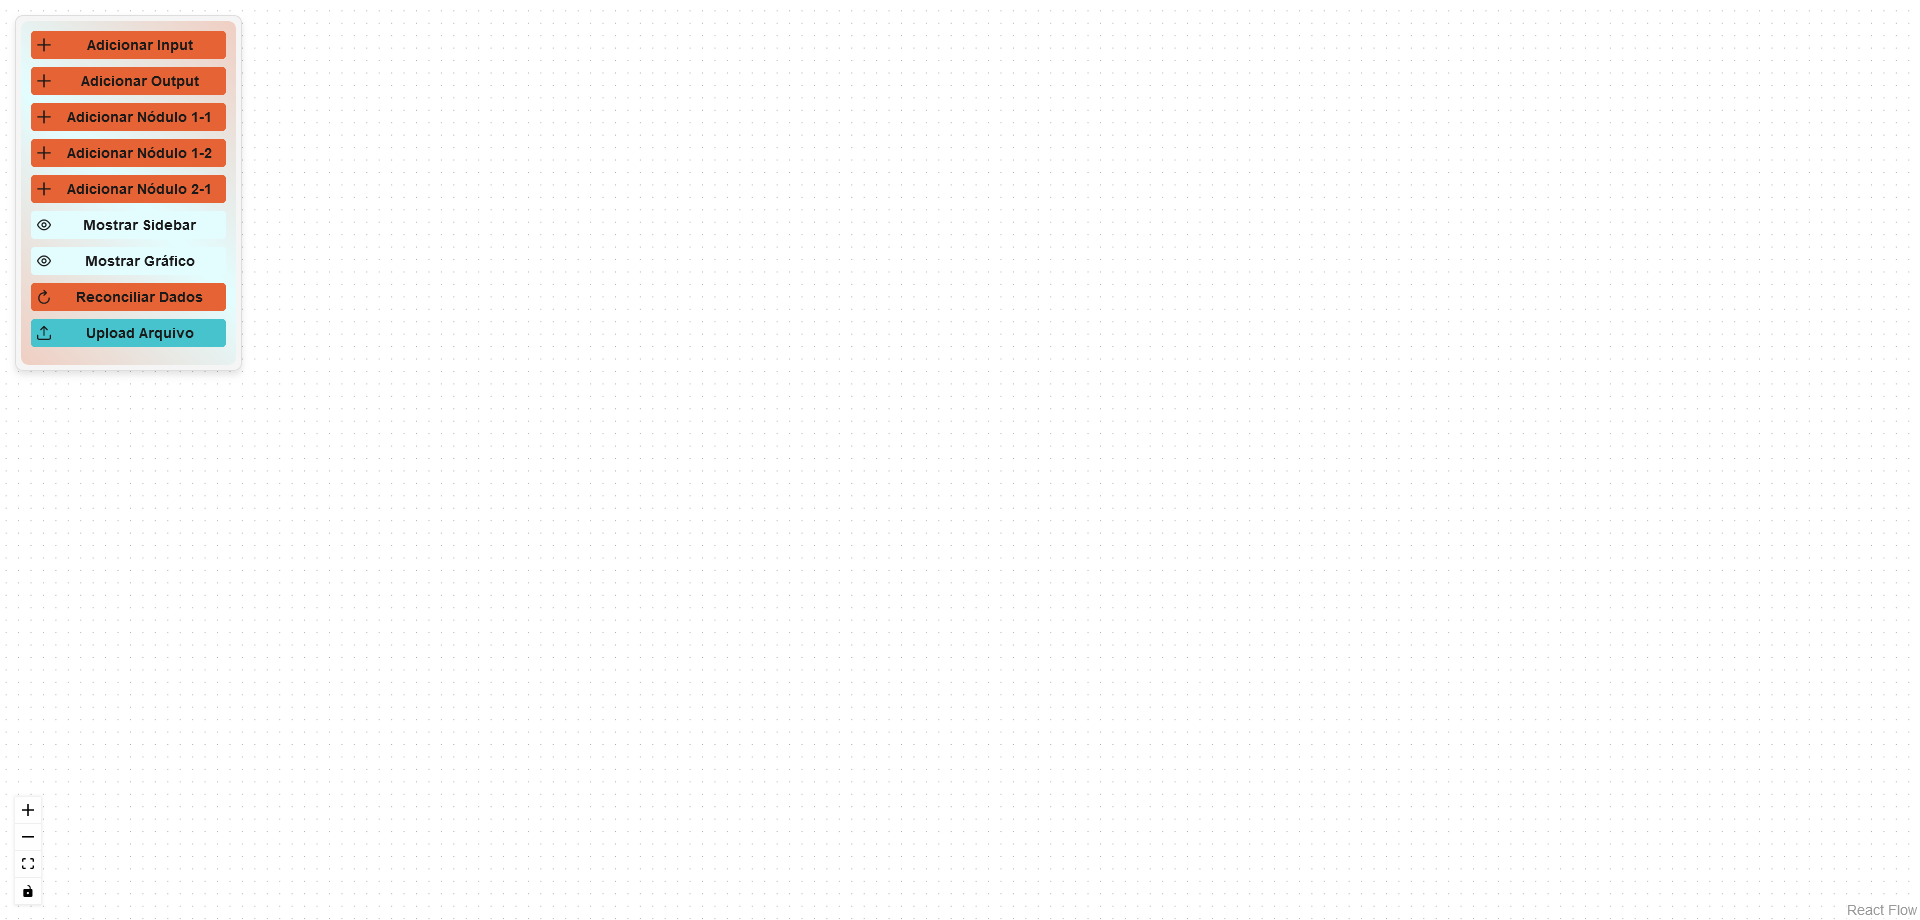
\includegraphics[width=0.8\textwidth]{figuras/empty-canvas.png}
    \caption{Exemplo da área de trabalho no canvas do RADARE (Fonte: próprio autor, 2024).}
    \label{Fig:CanvasArea}
\end{figure}

\subsubsection{Lógica de conexão entre os nódulos no \textit{canvas}}

O sistema permite que o usuário estabeleça conexões visuais entre os nódulos, representando o fluxo de dados entre diferentes pontos de um processo industrial. Essas conexões são fundamentais para garantir que os dados fluam corretamente entre os elementos do \textit{canvas}, como entradas, saídas e pontos de processamento.

A Figura \ref{Fig:NodeConnections} ilustra a conexão de dois nódulos no \textit{canvas}, demonstrando como o usuário pode arrastar e soltar as conexões de forma intuitiva. O usuário também pode ajustar e mover essas conexões entre os nódulos, proporcionando flexibilidade na organização dos fluxos de dados e permitindo a personalização do layout conforme as necessidades do processo.

O trecho principal do código responsável pela criação desse nódulo pode ser encontrado no \textbf{Apêndice \ref{Cap:frontCodeNodeTwoOne}}. Cada conexão entre os nódulos possui um valor e uma tolerância associados, que podem ser modificados diretamente com um duplo clique na linha de conexão. Isso permite ao usuário ajustar os parâmetros conforme necessário. Além disso, as conexões recebem nomes gerados automaticamente para facilitar a distinção entre as diferentes tags.

\begin{figure}[htbp]
    \centering
    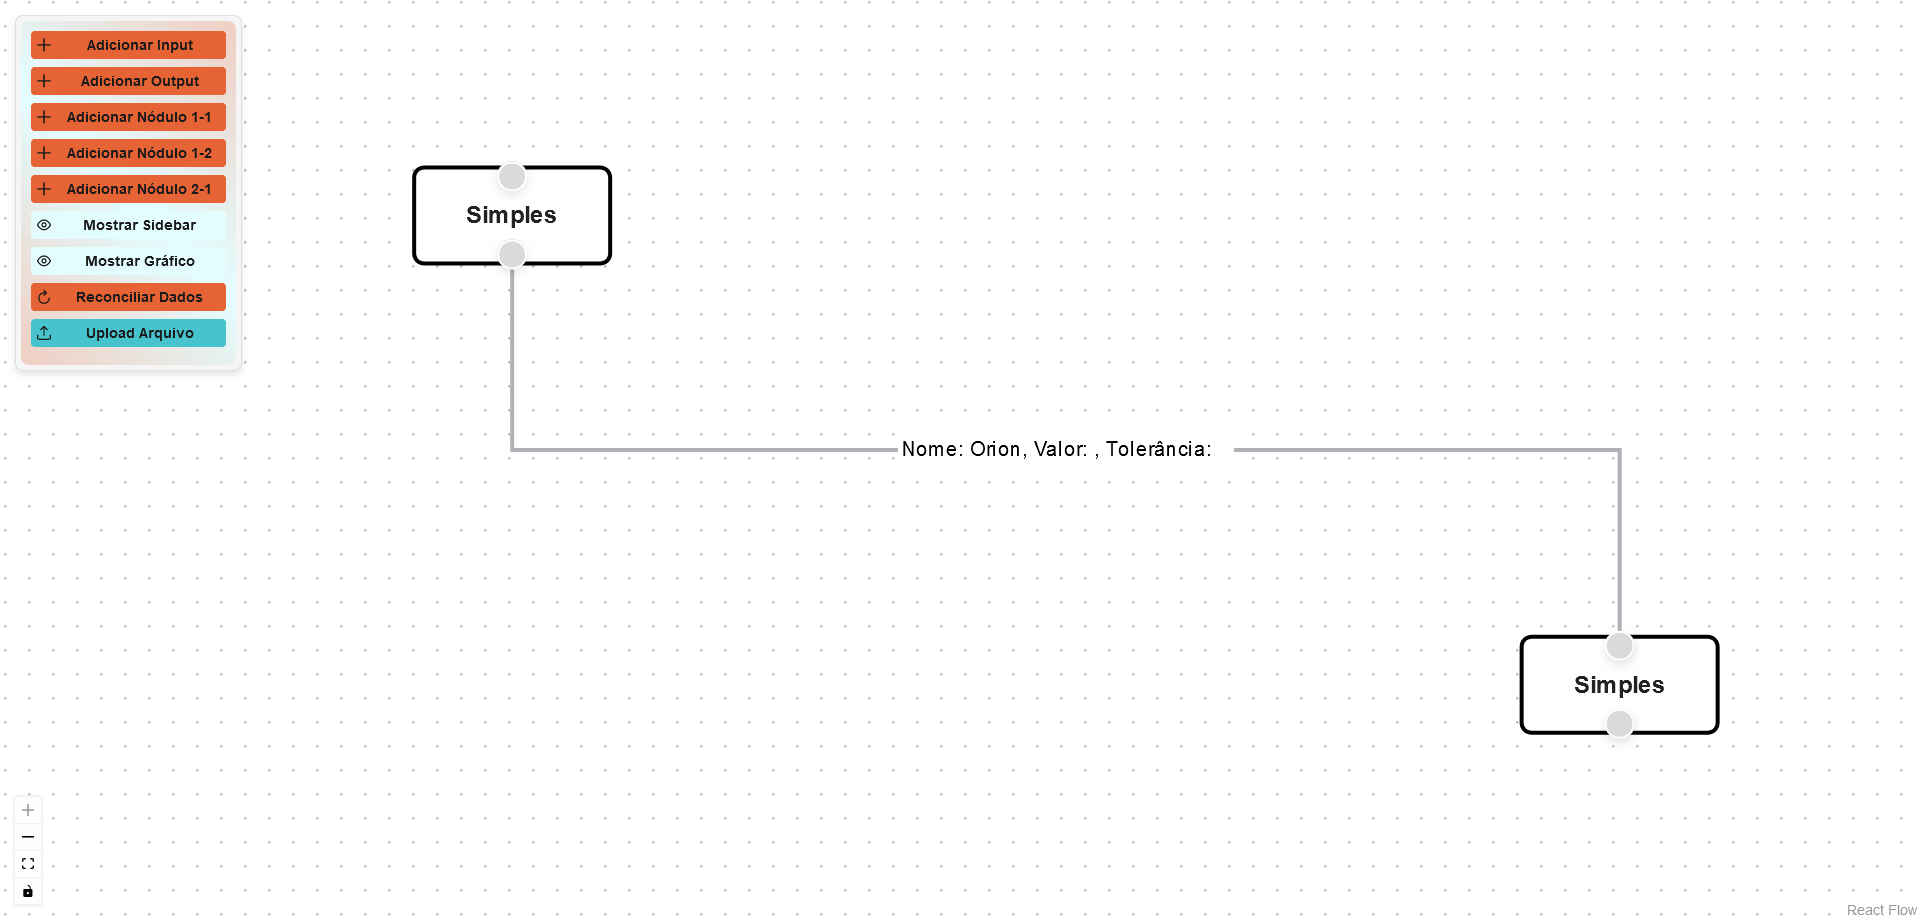
\includegraphics[width=0.8\textwidth]{figuras/node-connection-example.png}
    \caption{Exemplo de conexão entre nódulos no \textit{canvas} (Fonte: próprio autor, 2024).}
    \label{Fig:NodeConnections}
\end{figure}


% -------------------------
\subsection{Interface de gráfico de reconciliação de dados}

O \textit{canvas} é a área principal da interface do RADARE, onde o usuário pode visualizar, conectar e manipular os nódulos para configurar o fluxo de dados industrial. É nesse espaço que o usuário constrói e ajusta os fluxos de trabalho, interligando entradas, saídas e pontos de processamento. A interação no \textit{canvas} é dinâmica e permite a personalização dos fluxos conforme as necessidades do processo.

A Figura \ref{Fig:CanvasArea} mostra um exemplo do \textit{canvas} com vários nódulos conectados, oferecendo uma visão geral de como os elementos podem ser arranjados e manipulados visualmente. Nos próximos tópicos, exploraremos em detalhes as funcionalidades disponíveis no \textit{canvas}, com exemplos de código e explicações sobre a interação com os nódulos.

\begin{figure}[htbp]
    \centering
    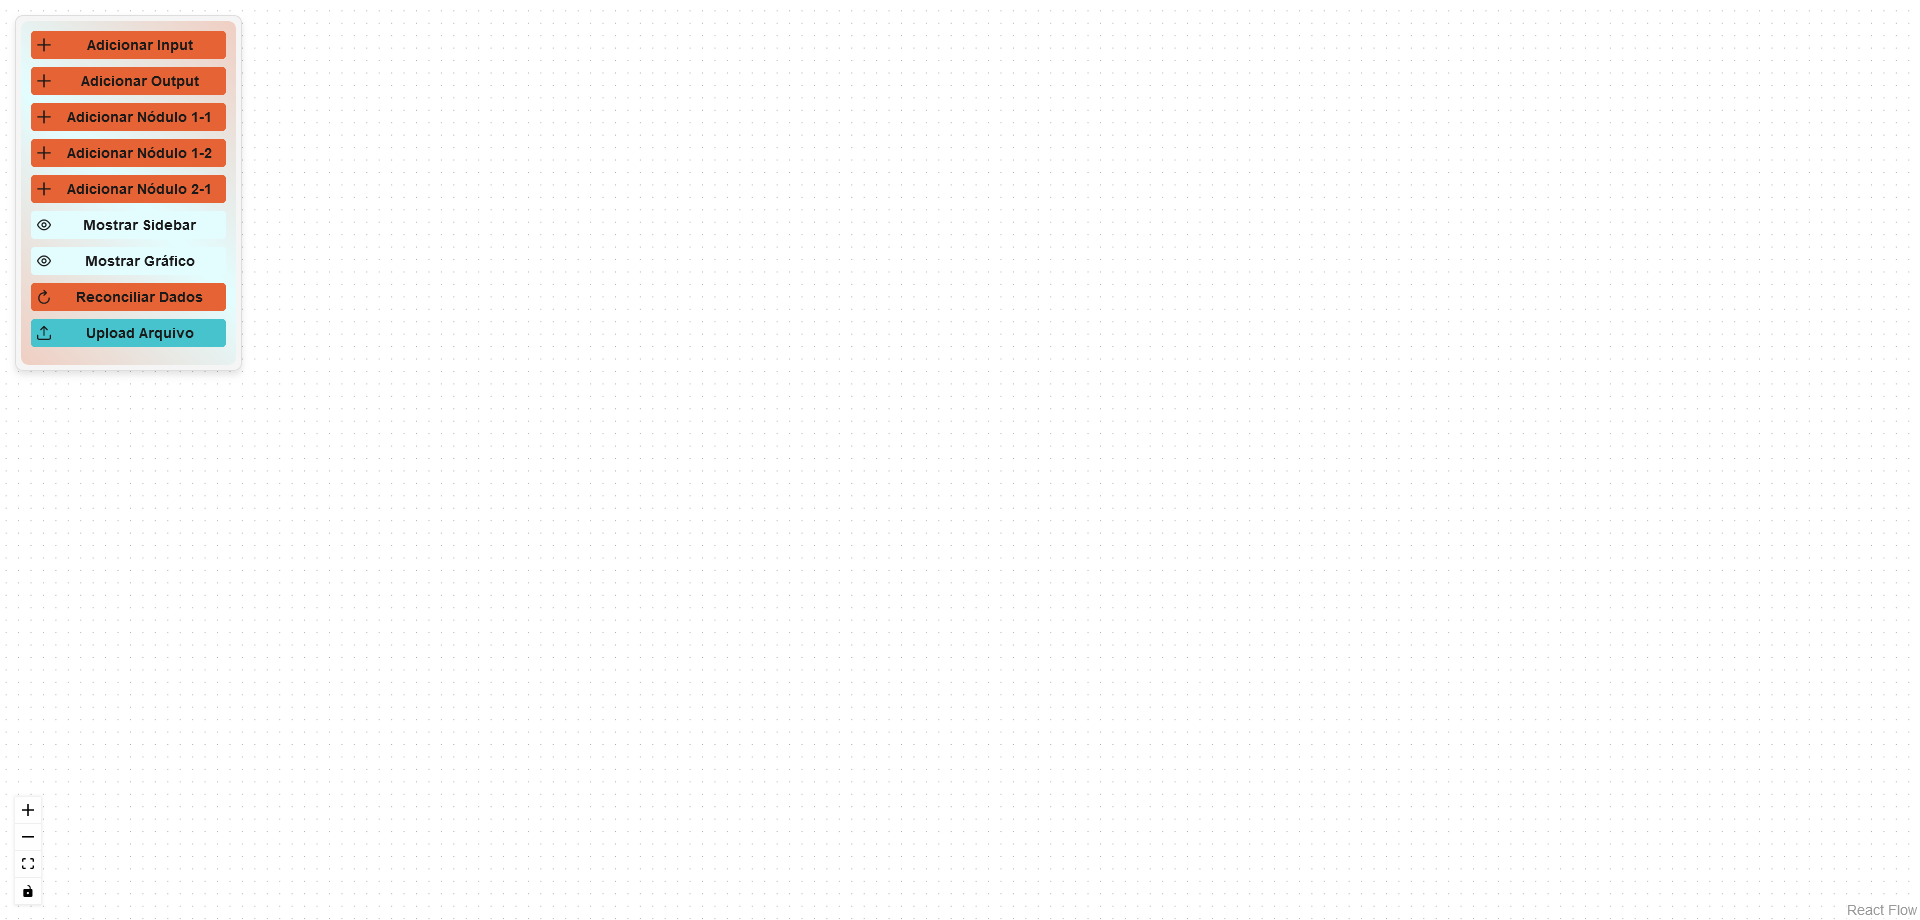
\includegraphics[width=0.8\textwidth]{figuras/empty-canvas.png}
    \caption{Exemplo da área de trabalho no canvas do RADARE (Fonte: próprio autor, 2024).}
    \label{Fig:CanvasArea}
\end{figure}


% -------------------------
\subsection{Interface de \textit{sidebar} de informações do sistema}

O \textit{canvas} é a área principal da interface do RADARE, onde o usuário pode visualizar, conectar e manipular os nódulos para configurar o fluxo de dados industrial. É nesse espaço que o usuário constrói e ajusta os fluxos de trabalho, interligando entradas, saídas e pontos de processamento. A interação no \textit{canvas} é dinâmica e permite a personalização dos fluxos conforme as necessidades do processo.

A Figura \ref{Fig:CanvasArea} mostra um exemplo do \textit{canvas} com vários nódulos conectados, oferecendo uma visão geral de como os elementos podem ser arranjados e manipulados visualmente. Nos próximos tópicos, exploraremos em detalhes as funcionalidades disponíveis no \textit{canvas}, com exemplos de código e explicações sobre a interação com os nódulos.

\begin{figure}[htbp]
    \centering
    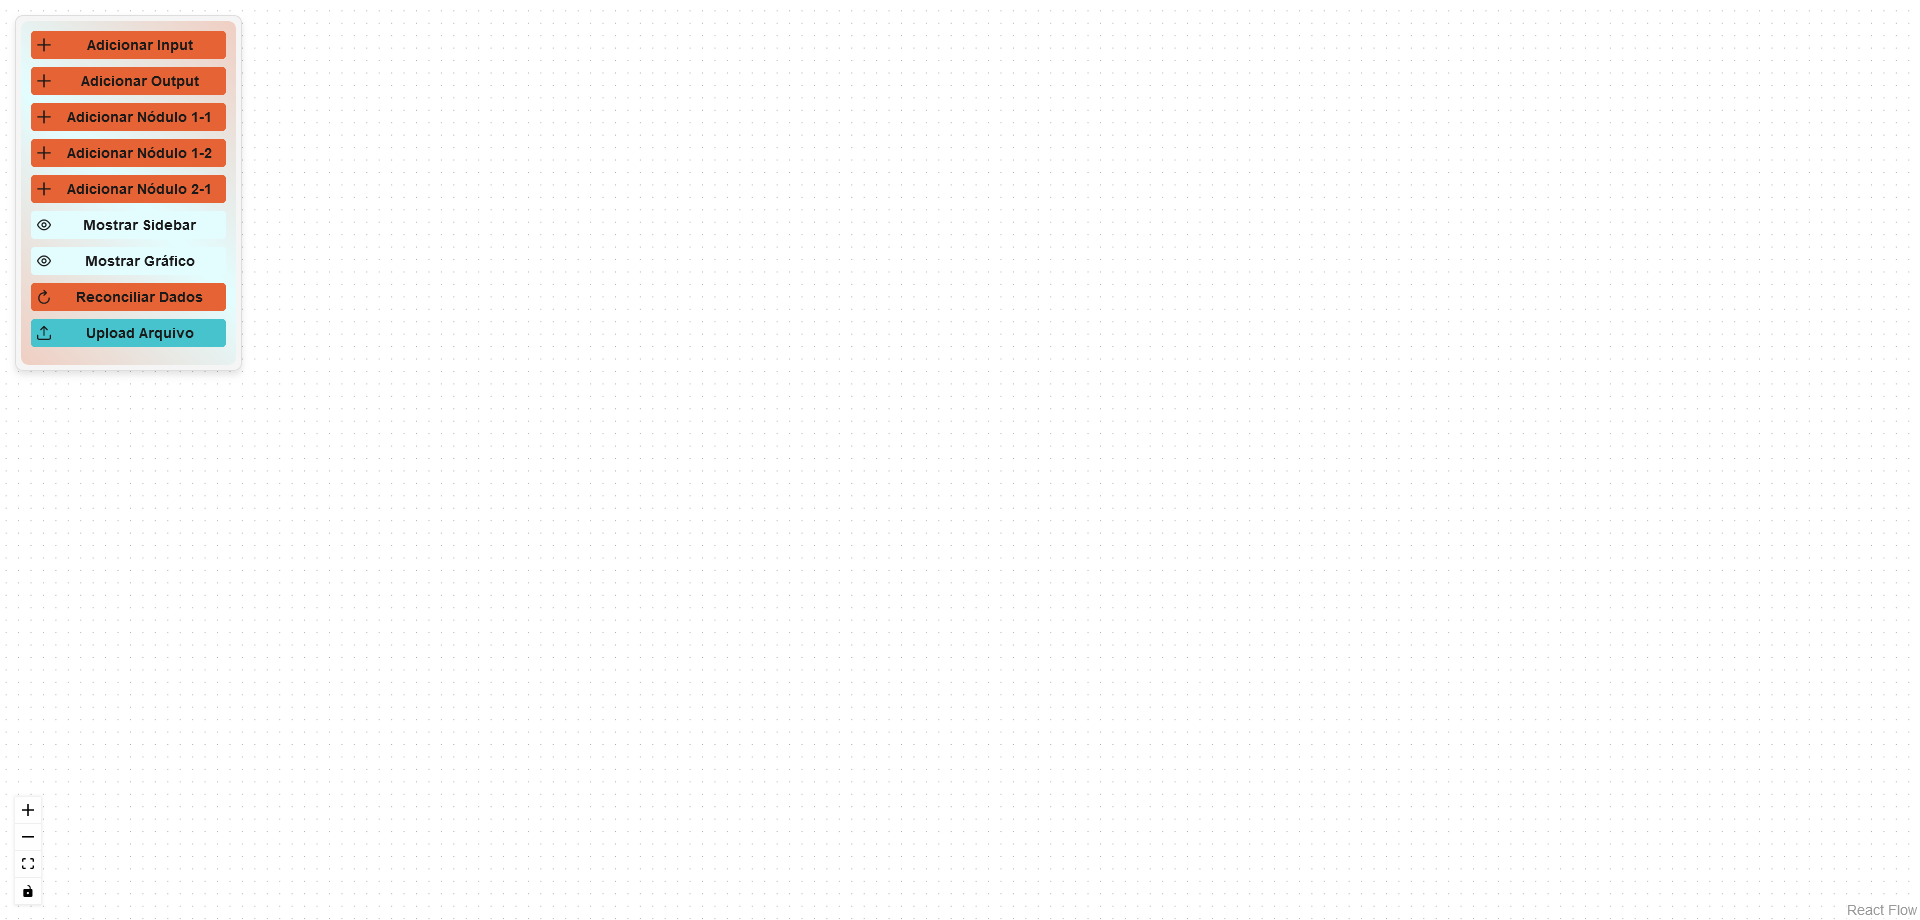
\includegraphics[width=0.8\textwidth]{figuras/empty-canvas.png}
    \caption{Exemplo da área de trabalho no canvas do RADARE (Fonte: próprio autor, 2024).}
    \label{Fig:CanvasArea}
\end{figure}

% -------------------------
\subsection{Resultados finais do front-end em sua visualização completa}

O \textit{canvas} é a área principal da interface do RADARE, onde o usuário pode visualizar, conectar e manipular os nódulos para configurar o fluxo de dados industrial. É nesse espaço que o usuário constrói e ajusta os fluxos de trabalho, interligando entradas, saídas e pontos de processamento. A interação no \textit{canvas} é dinâmica e permite a personalização dos fluxos conforme as necessidades do processo.

A Figura \ref{Fig:CanvasArea} apresenta um exemplo da área de trabalho do \textit{canvas} com vários nódulos conectados, permitindo uma visualização clara de como os elementos podem ser arranjados e manipulados visualmente. Cada nódulo representa uma função específica no processo, e as conexões entre eles ilustram o fluxo de dados que é tratado e reconciliado pelo sistema.

A seguir, exploraremos em detalhes as funcionalidades disponíveis no \textit{canvas}, incluindo a adição de nódulos, a conexão entre eles, a modificação de parâmetros, e a execução de tarefas de reconciliação de dados, sempre com exemplos práticos de código e interação no ambiente.

\begin{figure}[htbp]
    \centering
    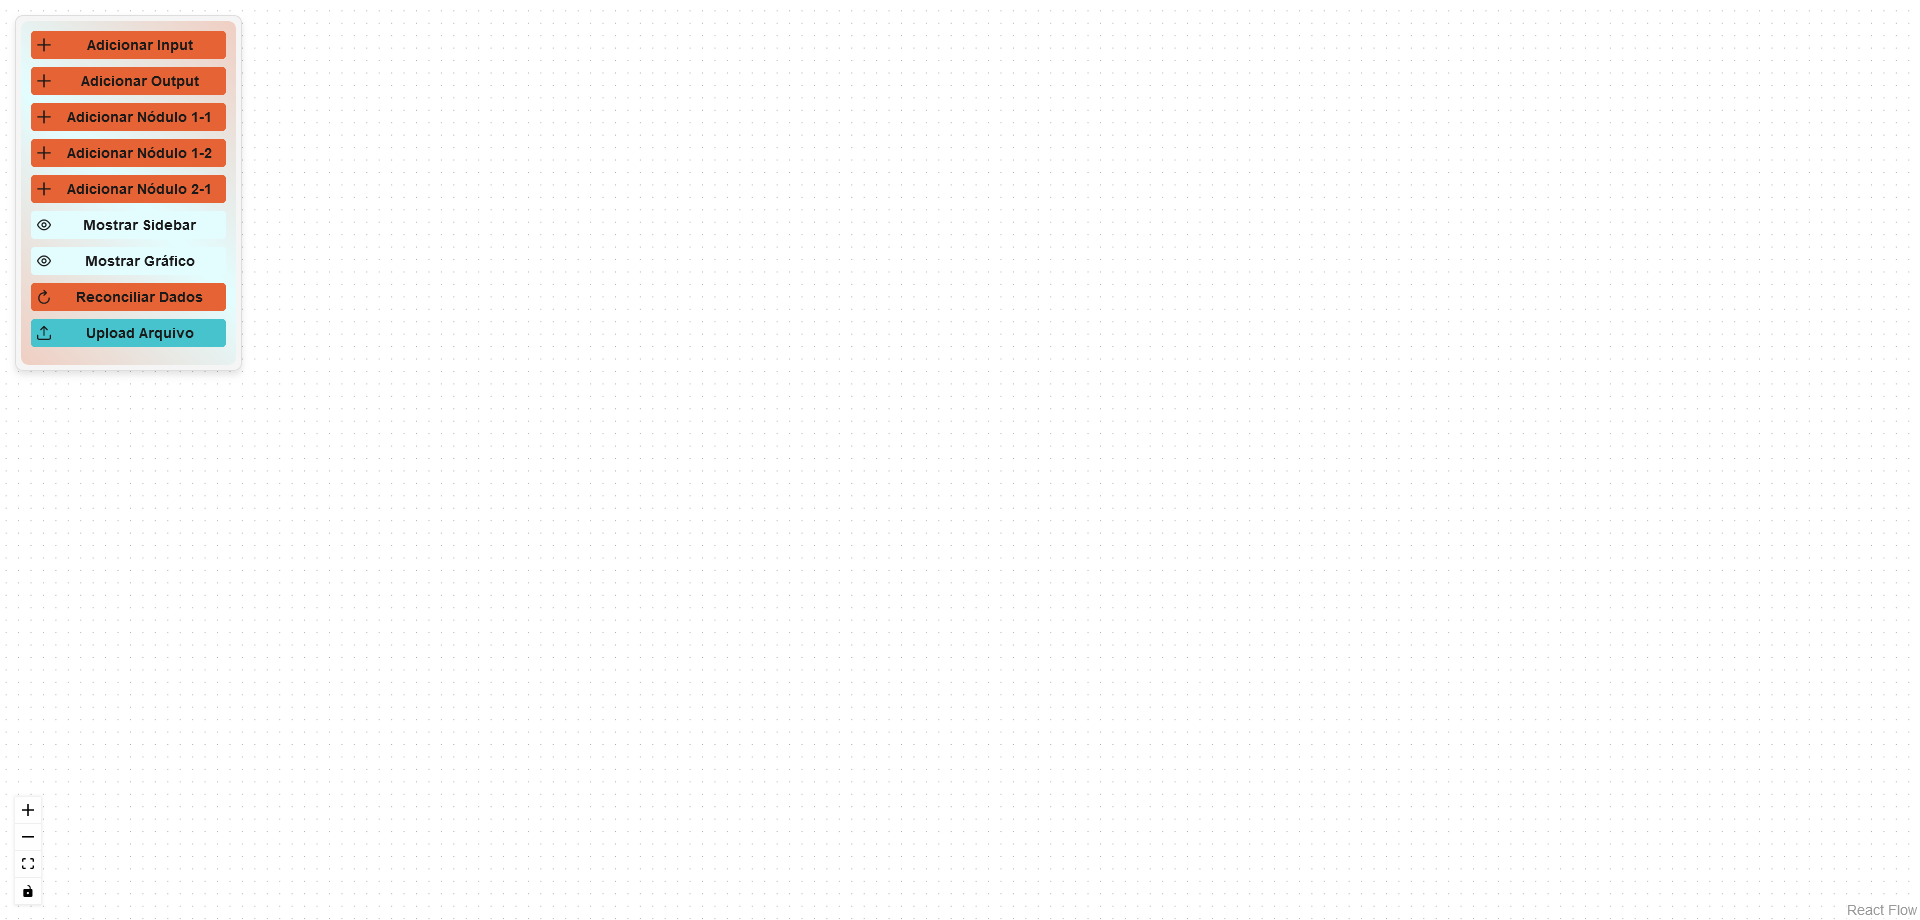
\includegraphics[width=0.8\textwidth]{figuras/empty-canvas.png}
    \caption{Exemplo da área de trabalho no canvas do RADARE (Fonte: próprio autor, 2024).}
    \label{Fig:CanvasArea}
\end{figure}

% -------------------------
\section{Resultados do desenvolvimento do \textit{back-end}}

O \textit{back-end} do RADARE foi desenvolvido em \textit{Python} utilizando o \textit{framework} Flask. Essa camada gerencia as requisições da interface, processa os dados submetidos pelo usuário e realiza os cálculos de reconciliação utilizando o método dos multiplicadores de Lagrange. A estrutura foi configurada para responder de maneira eficiente às operações do \textit{front-end}, enviando os resultados dos cálculos e garantindo uma comunicação ágil entre as partes do sistema.

Além de realizar a reconciliação de dados, o \textit{back-end} também gerencia a autenticação e o armazenamento seguro dos dados processados. Com essa estrutura, foi possível assegurar a integridade dos dados e a consistência nos processos realizados, resultando em um sistema robusto e preparado para operações contínuas e de alta demanda.

% -------------------------
\subsection{Desenvolvimento das interfaces RESTful de comunicação entre os sistemas}

As interfaces RESTful foram projetadas para garantir uma comunicação eficiente e segura entre o \textit{front-end} e o \textit{back-end} do sistema RADARE. Cada rota foi cuidadosamente estruturada para facilitar o envio e recebimento de dados, bem como a execução dos processos de reconciliação. Abaixo, são descritas as rotas implementadas, com exemplos de código e explicações detalhadas sobre cada funcionalidade, destacando a importância de cada \textit{endpoint} na integração dos componentes do sistema.

% -------------------------
\subsubsection{Interface RESTful POST /reconcile}

A rota \texttt{POST /reconcile} é responsável por receber os dados dos sensores enviados pelo \textit{front-end} e realizar a reconciliação utilizando o método dos multiplicadores de Lagrange. Após a entrada dos dados, o \textit{back-end} processa as informações e aplica o método para ajustar os valores conforme as restrições impostas, garantindo a consistência dos dados reconciliados. Os resultados obtidos são então armazenados no banco de dados, permitindo a sua recuperação e visualização pelo sistema conforme necessário.

O código completo que implementa essa funcionalidade pode ser consultado no \textbf{Anexo \ref{Anexo:CodigoRouteReconcile}}.

% -------------------------
\subsubsection{Interface RESTful GET /results}

A rota \texttt{GET /results} foi implementada para possibilitar que o usuário recupere os resultados das reconciliações de dados realizadas anteriormente. Ao ser acionada, essa rota consulta o banco de dados e retorna os valores reconciliados, que são então exibidos na interface gráfica, permitindo que o usuário visualize e analise os dados ajustados de forma clara e organizada.

O processo de recuperação desses dados envolve uma consulta ao banco de dados, onde as informações resultantes das reconciliações são armazenadas após o processamento inicial. Esses resultados incluem os valores corrigidos e ajustados por meio do método dos multiplicadores de Lagrange, aplicados durante a fase de reconciliação.

Para mais detalhes sobre o código completo desta rota, consulte o \textbf{Anexo \ref{Anexo:CodigoRouteResults}}, onde é apresentada a implementação completa, incluindo as especificidades da consulta ao banco de dados e a formatação dos dados antes de serem enviados para o \textit{front-end}.

% -------------------------
\subsubsection{Interface RESTful POST /upload}

A rota \texttt{POST /upload} é essencial para o funcionamento do RADARE, pois permite o envio de arquivos CSV contendo dados externos, como leituras de sensores industriais, que serão posteriormente integrados ao banco de dados do sistema. Esses dados servem de base para os processos de reconciliação, possibilitando uma análise precisa e consistente das informações coletadas.

Quando um arquivo é enviado através desta rota, ele é processado no \textit{back-end} para extrair as informações contidas no CSV. Em seguida, os dados são armazenados no banco de dados, ficando disponíveis para as etapas de reconciliação e visualização no \textit{front-end}. Esse fluxo garante que o sistema possa ser atualizado com dados de múltiplas fontes, permitindo uma integração contínua e ampliando a capacidade de análise do RADARE.

O código completo da implementação da rota \texttt{POST /upload} está disponível no \textbf{Anexo \ref{Anexo:CodigoRouteUpload}}.

% -------------------------
\subsection{Serviços}

Os serviços, comumente chamados de \textit{services} no \textit{back-end} são responsáveis por implementar a lógica de negócio, processar os dados e invocar os cálculos de reconciliação. Eles abstraem a complexidade do sistema, garantindo que os dados sejam processados corretamente antes de serem enviados ao banco de dados ou utilizados na interface. Abaixo estão descritos os principais \textit{services} do sistema RADARE, juntamente com exemplos de código e diagramas.


\subsubsection{Serviço de validação de dados}

A validação de dados garante que os dados recebidos estejam no formato correto antes de serem processados. Ele valida se todos os campos obrigatórios estão presentes, se os tipos de dados são consistentes e se não há valores ausentes ou inválidos.

O trecho principal do código responsável pela criação desse nódulo, que pode ser encontrado em sua totalidade no \textbf{Apêndice \ref{Cap:frontCodeNodeTwoOne}}.

\subsubsection{Serviço de processamento de dados}

O processamento de dados é responsável por lidar com arquivos CSV enviados pelos usuários. Ele converte os dados do arquivo em estruturas adequadas para o banco de dados e para os cálculos de reconciliação. Este serviço é crucial para integrar dados externos ao sistema RADARE.

O trecho principal do código responsável pela criação desse nódulo, que pode ser encontrado em sua totalidade no \textbf{Apêndice \ref{Cap:frontCodeNodeTwoOne}}.

\subsubsection{Serviço de reconciliação de dados}

A reconciliação de dados é o núcleo do sistema, responsável pela execução do algoritmo de reconciliação de dados. Ele aplica o método dos multiplicadores de Lagrange para garantir que as restrições de balanço de massa e energia sejam respeitadas durante a reconciliação dos dados.

O trecho principal do código responsável pela criação desse nódulo, que pode ser encontrado em sua totalidade no \textbf{Apêndice \ref{Cap:frontCodeNodeTwoOne}}.

\subsection{Models}

Os \textit{models} foram implementados utilizando \textit{Sequelize}, uma ORM (Object-Relational Mapping) para \textit{Node.js}, que facilita a comunicação com o banco de dados PostgreSQL. Os principais modelos incluem:

\begin{itemize} \item \textbf{Process Model}: Representa os processos industriais, contendo as informações de variáveis medidas e parâmetros. \item \textbf{Measurement Model}: Armazena as medições recebidas dos sensores. \item \textbf{Result Model}: Registra os resultados das reconciliações, vinculando-os aos processos e medições correspondentes. \end{itemize}

O trecho principal do código responsável pela criação desse nódulo, que pode ser encontrado em sua totalidade no \textbf{Apêndice \ref{Cap:frontCodeNodeTwoOne}}.

% -------------------------
\section{Resultados do desenvolvimento do banco de dados}

O banco de dados utilizado no sistema RADARE foi implementado em PostgreSQL e armazena todas as informações relevantes para a execução do processo de reconciliação de dados industriais, gerenciamento de usuários e rastreamento de atividades. A modelagem foi feita de forma a garantir a integridade e eficiência na consulta e manipulação dos dados. A seguir, são descritas as principais tabelas implementadas no sistema.

\subsection{Tabela de Dados de Processos}

A tabela que armazena os dados de processos industriais contém as medições e os resultados da reconciliação. As principais colunas são:

\begin{itemize}
    \item \textbf{id}: Coluna de identificação única para cada registro no banco de dados. Utilizada como chave primária para vincular informações em diferentes tabelas.
    \item \textbf{user}: Armazena informações sobre o usuário que realizou o upload dos dados ou a operação de reconciliação.
    \item \textbf{time}: Representa o timestamp associado ao dado, indicando o momento exato em que a medição foi realizada ou quando a reconciliação foi executada.
    \item \textbf{tagname}: Identifica a variável medida (sensor ou ponto de coleta) no processo industrial. Cada variável é referenciada por um nome único.
    \item \textbf{tagreconciled}: Armazena o valor reconciliado de cada variável, ou seja, o resultado do processo de reconciliação de dados.
    \item \textbf{tagcorrection}: Coluna que contém o valor da correção aplicada a cada variável medida.
    \item \textbf{tagmatrix}: Refere-se à matriz de correlação utilizada no processo de reconciliação.
\end{itemize}

\subsection{Tabela de Usuários}

Esta tabela gerencia a autenticação e as permissões dos usuários no sistema. Ela permite o rastreamento de interações e garante que apenas usuários autorizados possam realizar determinadas operações, além de armazenar informações para autenticação segura.

\begin{table}[htbp]
    \centering
    \caption{Estrutura da tabela de usuários.}
    \label{Tab:Users}
    \begin{tabular}{|c|c|}
        \hline
        \textbf{Coluna} & \textbf{Descrição} \\ \hline
        id (primary key) & UUID único para cada usuário \\ \hline
        username & Nome de usuário utilizado no login \\ \hline
        email & Email do usuário para notificações e recuperação de senha \\ \hline
        password\_hash & Hash da senha para garantir segurança \\ \hline
        role & Papel do usuário (admin, operador, analista) \\ \hline
        created\_at & Timestamp da criação da conta \\ \hline
        last\_login & Data e hora do último login realizado \\ \hline
    \end{tabular}
\end{table}

\subsection{Tabela de Logs de Atividade}

Esta tabela registra as ações realizadas pelos usuários no sistema, permitindo auditoria e rastreamento de atividades como uploads de arquivos ou execuções de reconciliação de dados.

\begin{table}[htbp]
    \centering
    \caption{Estrutura da tabela de logs de atividade.}
    \label{Tab:ActivityLogs}
    \begin{tabular}{|c|c|}
        \hline
        \textbf{Coluna} & \textbf{Descrição} \\ \hline
        id (primary key) & Identificação única para cada log de atividade \\ \hline
        user\_id & Referência ao id do usuário que realizou a ação \\ \hline
        action & Descrição da ação realizada (ex: upload de CSV, reconciliação de dados) \\ \hline
        timestamp & Data e hora em que a ação foi realizada \\ \hline
        details & Detalhes adicionais sobre a ação (ex: nome do arquivo CSV carregado) \\ \hline
    \end{tabular}
\end{table}

\subsection{Tabela de Configurações de Processos}

Esta tabela armazena as configurações dos processos industriais, incluindo parâmetros como limites de variáveis e tipos de medições. Essa estrutura permite personalizar o comportamento do sistema para diferentes cenários industriais.

\begin{table}[htbp]
    \centering
    \caption{Estrutura da tabela de configurações de processos.}
    \label{Tab:ProcessConfigurations}
    \begin{tabular}{|c|c|}
        \hline
        \textbf{Coluna} & \textbf{Descrição} \\ \hline
        id (primary key) & Identificação única para a configuração do processo \\ \hline
        process\_name & Nome do processo industrial \\ \hline
        sensor\_limits & Limites definidos para as variáveis dos sensores \\ \hline
        created\_by & ID do usuário que criou a configuração \\ \hline
        created\_at & Timestamp de criação da configuração \\ \hline
    \end{tabular}
\end{table}

Essa modelagem de banco de dados garante rastreabilidade, segurança e eficiência no gerenciamento de processos industriais e usuários dentro do sistema RADARE.

% -------------------------
\section{Manuais de sistema}

Como parte do desenvolvimento do \textit{software} RADARE, foram criados dois manuais distintos para auxiliar tanto os administradores técnicos quanto os usuários finais na utilização e manutenção do sistema. Esses manuais visam garantir a correta operação e longevidade da aplicação, fornecendo instruções claras sobre o funcionamento do sistema e as melhores práticas para sua utilização.

\subsection{Manual de manutenção do sistema}

O manual de manutenção do sistema foi elaborado para orientar desenvolvedores e administradores sobre as funções internas do RADARE, assim como as restrições e considerações técnicas envolvidas. Ele oferece uma visão detalhada da arquitetura do sistema, explicando cada módulo, como o *front-end*, *back-end* e banco de dados, além de descrever as principais funções, fluxos de dados e interações entre os componentes. O manual também fornece instruções para realizar tarefas de manutenção, como atualização de bibliotecas, ajustes de configurações, monitoramento de logs e execução de testes de desempenho. São abordadas as limitações técnicas do sistema, incluindo o número máximo de conexões simultâneas suportadas, tamanhos máximos de arquivos *CSV* e requisitos mínimos de hardware e software. Além disso, o manual traz procedimentos detalhados para diagnosticar e resolver possíveis problemas, como erros de reconciliação, falhas no processamento de arquivos e dificuldades de conexão entre os módulos. 

O manual completo com todos os detalhes estará disponível no \textbf{Apêndice \ref{Cap:manualManutencao}}, facilitando o acesso e consulta a informações detalhadas sobre a manutenção do sistema.

\subsection{Manual de uso para o usuário final}

O manual de uso foi criado com o objetivo de fornecer ao usuário comum uma orientação simples e direta sobre como utilizar o *RADARE* para realizar tarefas cotidianas de reconciliação de dados industriais. Ele inclui uma introdução ao sistema, explicando o propósito do *RADARE*, suas funcionalidades principais e como ele pode contribuir para a melhoria da qualidade dos dados nos processos industriais. Em seguida, apresenta um passo a passo detalhado de operações, com instruções sobre como utilizar cada parte da interface, como adicionar nódulos no *canvas*, realizar reconciliações de dados e carregar arquivos *CSV*.

O manual também oferece guias visuais com imagens ilustrativas que mostram o processo de navegação na interface, desde a adição de nódulos até a geração de gráficos de reconciliação. Há dicas de usabilidade que ajudam a utilizar a ferramenta de maneira mais eficiente, sugerindo atalhos, formas de personalizar fluxos de trabalho e como maximizar a utilidade dos relatórios gerados. Além disso, inclui uma seção de resolução de problemas comuns, abordando erros de upload de arquivos, falhas na conexão entre nódulos e dificuldades na interpretação dos resultados.

Este manual foi projetado para ser acessível a usuários com diferentes níveis de habilidade técnica, facilitando o uso do *RADARE* de forma intuitiva e prática no dia a dia. O manual completo pode ser consultado no \textbf{Apêndice \ref{Cap:manualUsuario}}, onde são fornecidos todos os detalhes e instruções.